\documentclass[14pt]{extbook}
\usepackage{multicol, enumerate, enumitem, hyperref, color, soul, setspace, parskip, fancyhdr} %General Packages
\usepackage{amssymb, amsthm, amsmath, bbm, latexsym, units, mathtools} %Math Packages
\everymath{\displaystyle} %All math in Display Style
% Packages with additional options
\usepackage[headsep=0.5cm,headheight=12pt, left=1 in,right= 1 in,top= 1 in,bottom= 1 in]{geometry}
\usepackage[usenames,dvipsnames]{xcolor}
\usepackage{dashrule}  % Package to use the command below to create lines between items
\newcommand{\litem}[1]{\item#1\hspace*{-1cm}\rule{\textwidth}{0.4pt}}
\pagestyle{fancy}
\lhead{Makeup Progress Quiz 1}
\chead{}
\rhead{Version A}
\lfoot{6018-3080}
\cfoot{}
\rfoot{Spring 2021}
\begin{document}

\begin{enumerate}
\litem{
Solve the radical equation below. Then, choose the interval(s) that the solution(s) belongs to.\[ \sqrt{-6 x + 3} - \sqrt{4 x + 9} = 0 \]\begin{enumerate}[label=\Alph*.]
\item \( x_1 \in [-0.7, 0.4] \text{ and } x_2 \in [-0.5,4.5] \)
\item \( x_1 \in [-2.8, -1.8] \text{ and } x_2 \in [-0.5,4.5] \)
\item \( x \in [0.5,2.2] \)
\item \( x \in [-0.7,0.4] \)
\item \( \text{All solutions lead to invalid or complex values in the equation.} \)

\end{enumerate} }
\litem{
What is the domain of the function below?\[ f(x) = \sqrt[3]{-8 x - 5} \]\begin{enumerate}[label=\Alph*.]
\item \( \text{The domain is } (-\infty, a], \text{   where } a \in [-2.4, -0.78] \)
\item \( \text{The domain is } [a, \infty), \text{   where } a \in [-2.22, -0.98] \)
\item \( (-\infty, \infty) \)
\item \( \text{The domain is } [a, \infty), \text{   where } a \in [-0.78, -0.1] \)
\item \( \text{The domain is } (-\infty, a], \text{   where } a \in [-1.13, -0.6] \)

\end{enumerate} }
\litem{
Choose the graph of the equation below.\[ f(x) = - \sqrt{x + 14} + 3 \]\begin{enumerate}[label=\Alph*.]
\begin{multicols}{2}\item 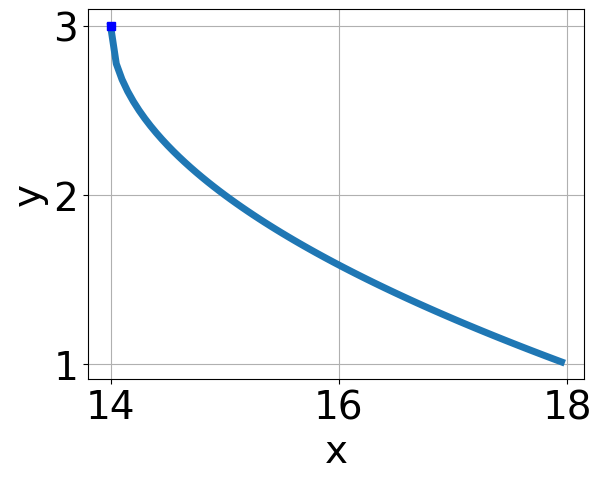
\includegraphics[width = 0.3\textwidth]{../Figures/radicalEquationToGraphAA.png}\item 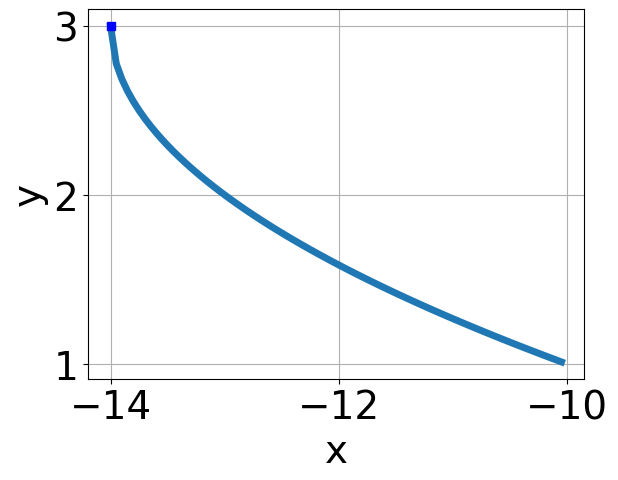
\includegraphics[width = 0.3\textwidth]{../Figures/radicalEquationToGraphBA.png}\item 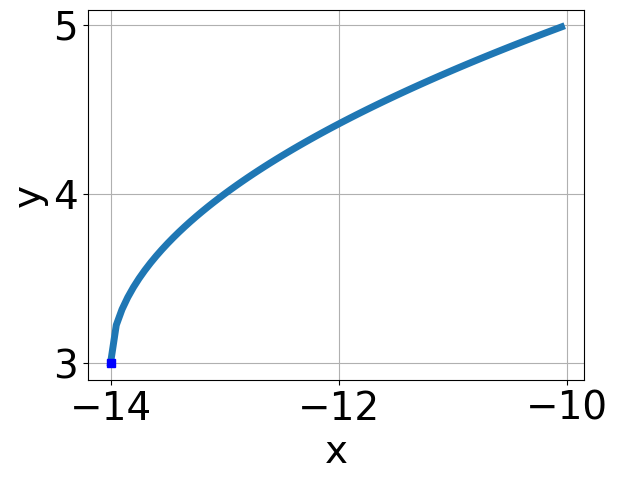
\includegraphics[width = 0.3\textwidth]{../Figures/radicalEquationToGraphCA.png}\item 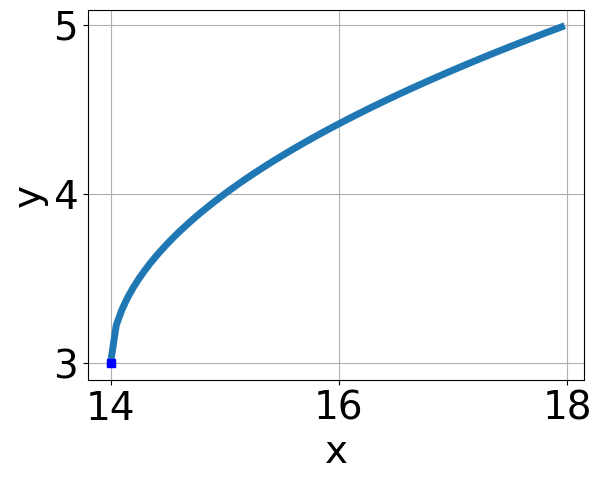
\includegraphics[width = 0.3\textwidth]{../Figures/radicalEquationToGraphDA.png}\end{multicols}\item None of the above.
\end{enumerate} }
\litem{
Solve the radical equation below. Then, choose the interval(s) that the solution(s) belongs to.\[ \sqrt{-30 x^2 - 32} - \sqrt{-64 x} = 0 \]\begin{enumerate}[label=\Alph*.]
\item \( x_1 \in [0.49, 1.08] \text{ and } x_2 \in [-0.67,3.33] \)
\item \( \text{All solutions lead to invalid or complex values in the equation.} \)
\item \( x \in [1.08,2.63] \)
\item \( x \in [0.49,1.08] \)
\item \( x_1 \in [-2.39, -0.64] \text{ and } x_2 \in [-2.33,0.67] \)

\end{enumerate} }
\litem{
Choose the equation of the function graphed below.
\begin{center}
    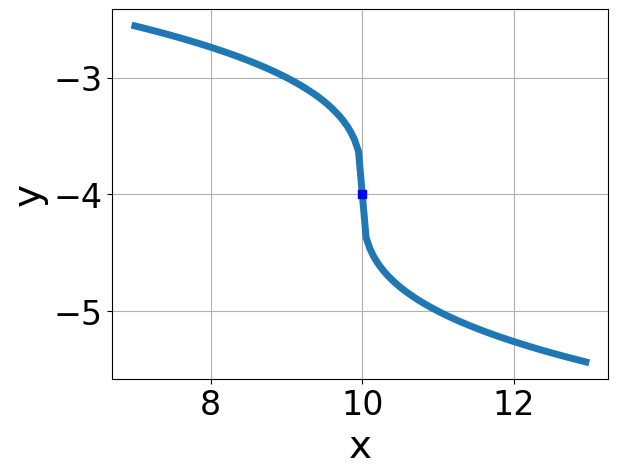
\includegraphics[width=0.5\textwidth]{../Figures/radicalGraphToEquationCopyA.png}
\end{center}
\begin{enumerate}[label=\Alph*.]
\item \( f(x) = - \sqrt{x + 10} - 4 \)
\item \( f(x) = \sqrt{x + 10} - 4 \)
\item \( f(x) = \sqrt{x - 10} - 4 \)
\item \( f(x) = - \sqrt{x - 10} - 4 \)
\item \( \text{None of the above} \)

\end{enumerate} }
\litem{
What is the domain of the function below?\[ f(x) = \sqrt[6]{3 x - 5} \]\begin{enumerate}[label=\Alph*.]
\item \( (-\infty, a], \text{where } a \in [-3.4, 1.6] \)
\item \( [a, \infty), \text{ where } a \in [1.47, 2.68] \)
\item \( (-\infty, a], \text{where } a \in [0.67, 5.67] \)
\item \( [a, \infty), \text{where } a \in [-0.17, 0.77] \)
\item \( (-\infty, \infty) \)

\end{enumerate} }
\litem{
Solve the radical equation below. Then, choose the interval(s) that the solution(s) belongs to.\[ \sqrt{35 x^2 + 15} - \sqrt{50 x} = 0 \]\begin{enumerate}[label=\Alph*.]
\item \( \text{All solutions lead to invalid or complex values in the equation.} \)
\item \( x \in [0.88,1.16] \)
\item \( x \in [0.06,0.85] \)
\item \( x_1 \in [-1.28, -0.72] \text{ and } x_2 \in [-2.43,0.57] \)
\item \( x_1 \in [0.06, 0.85] \text{ and } x_2 \in [1,4] \)

\end{enumerate} }
\litem{
Choose the equation of the function graphed below.
\begin{center}
    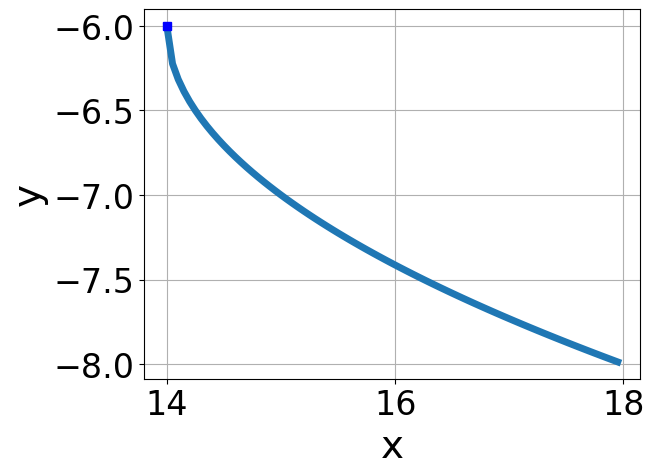
\includegraphics[width=0.5\textwidth]{../Figures/radicalGraphToEquationA.png}
\end{center}
\begin{enumerate}[label=\Alph*.]
\item \( f(x) = \sqrt[3]{x + 14} - 6 \)
\item \( f(x) = - \sqrt[3]{x + 14} - 6 \)
\item \( f(x) = \sqrt[3]{x - 14} - 6 \)
\item \( f(x) = - \sqrt[3]{x - 14} - 6 \)
\item \( \text{None of the above} \)

\end{enumerate} }
\litem{
Solve the radical equation below. Then, choose the interval(s) that the solution(s) belongs to.\[ \sqrt{7 x - 5} - \sqrt{5 x - 4} = 0 \]\begin{enumerate}[label=\Alph*.]
\item \( x \in [4.44,4.64] \)
\item \( \text{All solutions lead to invalid or complex values in the equation.} \)
\item \( x_1 \in [0.34, 0.68] \text{ and } x_2 \in [0.61,0.72] \)
\item \( x_1 \in [0.63, 1.12] \text{ and } x_2 \in [0.72,0.96] \)
\item \( x \in [0.34,0.68] \)

\end{enumerate} }
\litem{
Choose the graph of the equation below.\[ f(x) = - \sqrt[3]{x + 8} + 5 \]\begin{enumerate}[label=\Alph*.]
\begin{multicols}{2}\item 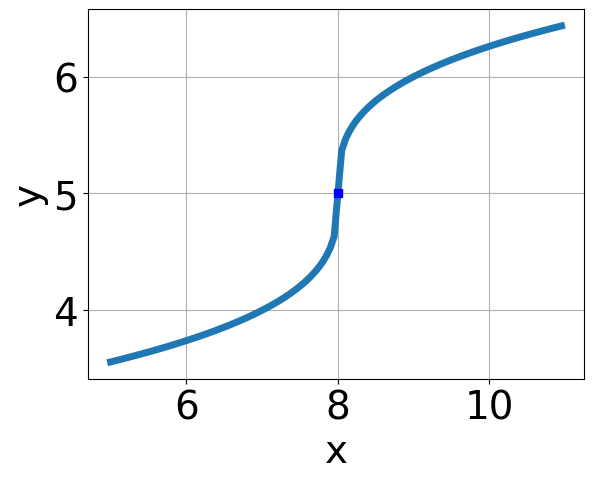
\includegraphics[width = 0.3\textwidth]{../Figures/radicalEquationToGraphCopyAA.png}\item 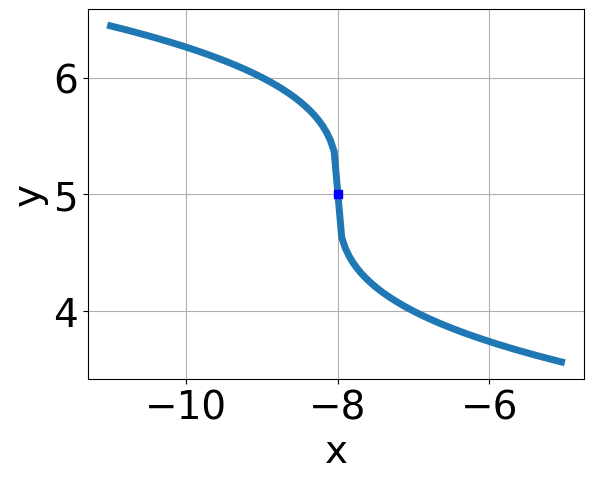
\includegraphics[width = 0.3\textwidth]{../Figures/radicalEquationToGraphCopyBA.png}\item 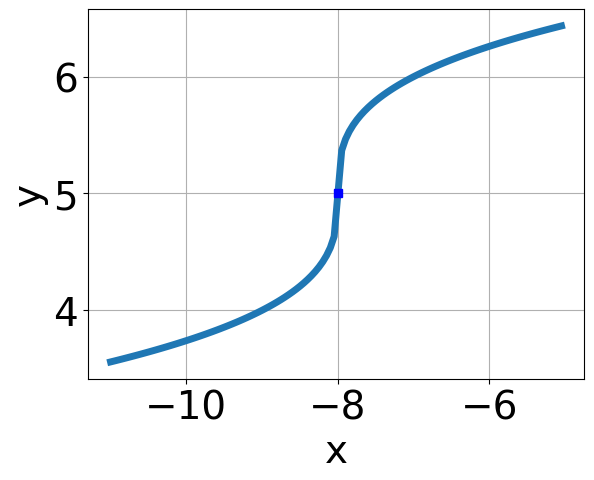
\includegraphics[width = 0.3\textwidth]{../Figures/radicalEquationToGraphCopyCA.png}\item 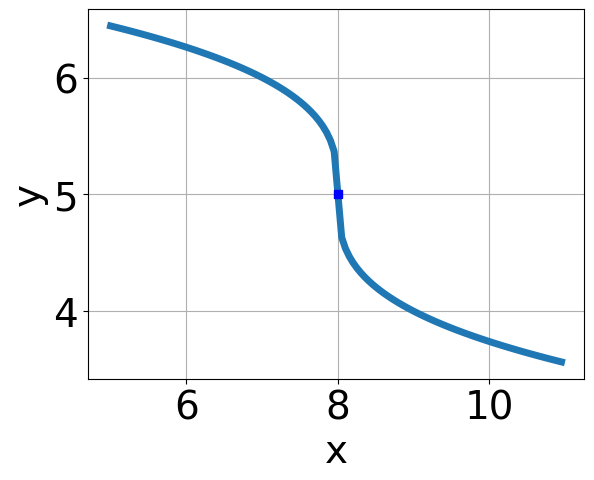
\includegraphics[width = 0.3\textwidth]{../Figures/radicalEquationToGraphCopyDA.png}\end{multicols}\item None of the above.
\end{enumerate} }
\end{enumerate}

\end{document}